\section{Start/Stop StarRiver
Service}\label{startstop-starriver-service}

StarRiver Server runs in background as a service. You could manually
start or stop the service via shortcuts in Start Menu.

\begin{figure}[htbp]
\centering
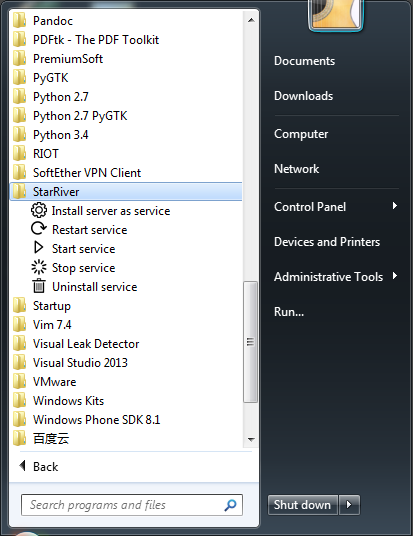
\includegraphics{img/shortcuts.png}
\end{figure}

Five shortcuts created during installation are:

\begin{itemize}
\itemsep1pt\parskip0pt\parsep0pt
\item
  \textbf{Install server as service}: Install StarRiver Server as a
  Windows service. This has been done during installation.
\item
  \textbf{Restart service}: Manually restart StarRiver service.
\item
  \textbf{Start service}: Manually start StarRiver service.
\item
  \textbf{Stop service}: Manually stop StarRiver service.
\item
  \textbf{Uninstall service}: Remove the StarRiver Windows service.
  StarRiver communication application will not be removed. But it will
  no longer starts with the system.
\end{itemize}
